\section{Trabalhos Relacionados}

Durante a pesquisa bibliográfica realizada neste trabalho, encontrou-se alguns trabalhos que também fizeram análise de textos parlamentares utilizando aprendizado bayesiano. O Retórica Parlamentar\footnote{http://retorica.labhackercd.net/about.html}, idealizado por Davi Moreira\footnote{https://github.com/davi-moreira}, Manoel Galdino\footnote{https://github.com/mgaldino} e Luis Carli\footnote{https://github.com/luiscarli}, utiliza os discursos proferidos pelos parlamentares no Pequeno Expediente e no Grande Expediente da Câmara dos Deputados para promover a transparência do mandato e fornecer subsídios para o controle social com a divulgação dos temas mais debatidos em Plenário.

A técnica utilizada pelo Retórica para a classificação dos discursos é um modelo bayesiano hierárquico, descrito por \citeonline{grimmer2009}, onde através de aprendizado não supervisionado são gerados \(k\) \textit{clusters}, sendo \(k\) um valor escolhido ao executar o algoritmo. O resultado é exportado para o formato \textit{csv} e contém os termos mais frequentes de cada cluster. Em seguida, um especialista deve ler e rotular cada \textit{cluster}.

A visualização dos dados é feita através de um gráfico de bolhas, em que cada bolha representa a relevância (medida pela frequência) de cada tema dentre todos os deputados analisados. Dentro de cada bolha são colocados os deputados que enfatizam aquele tema nos seus discursos. Um deputado está associado a um único tema, que é o tema mais enfatizado por ele nos seus discursos.

\begin{figure}[h]
    \centering
    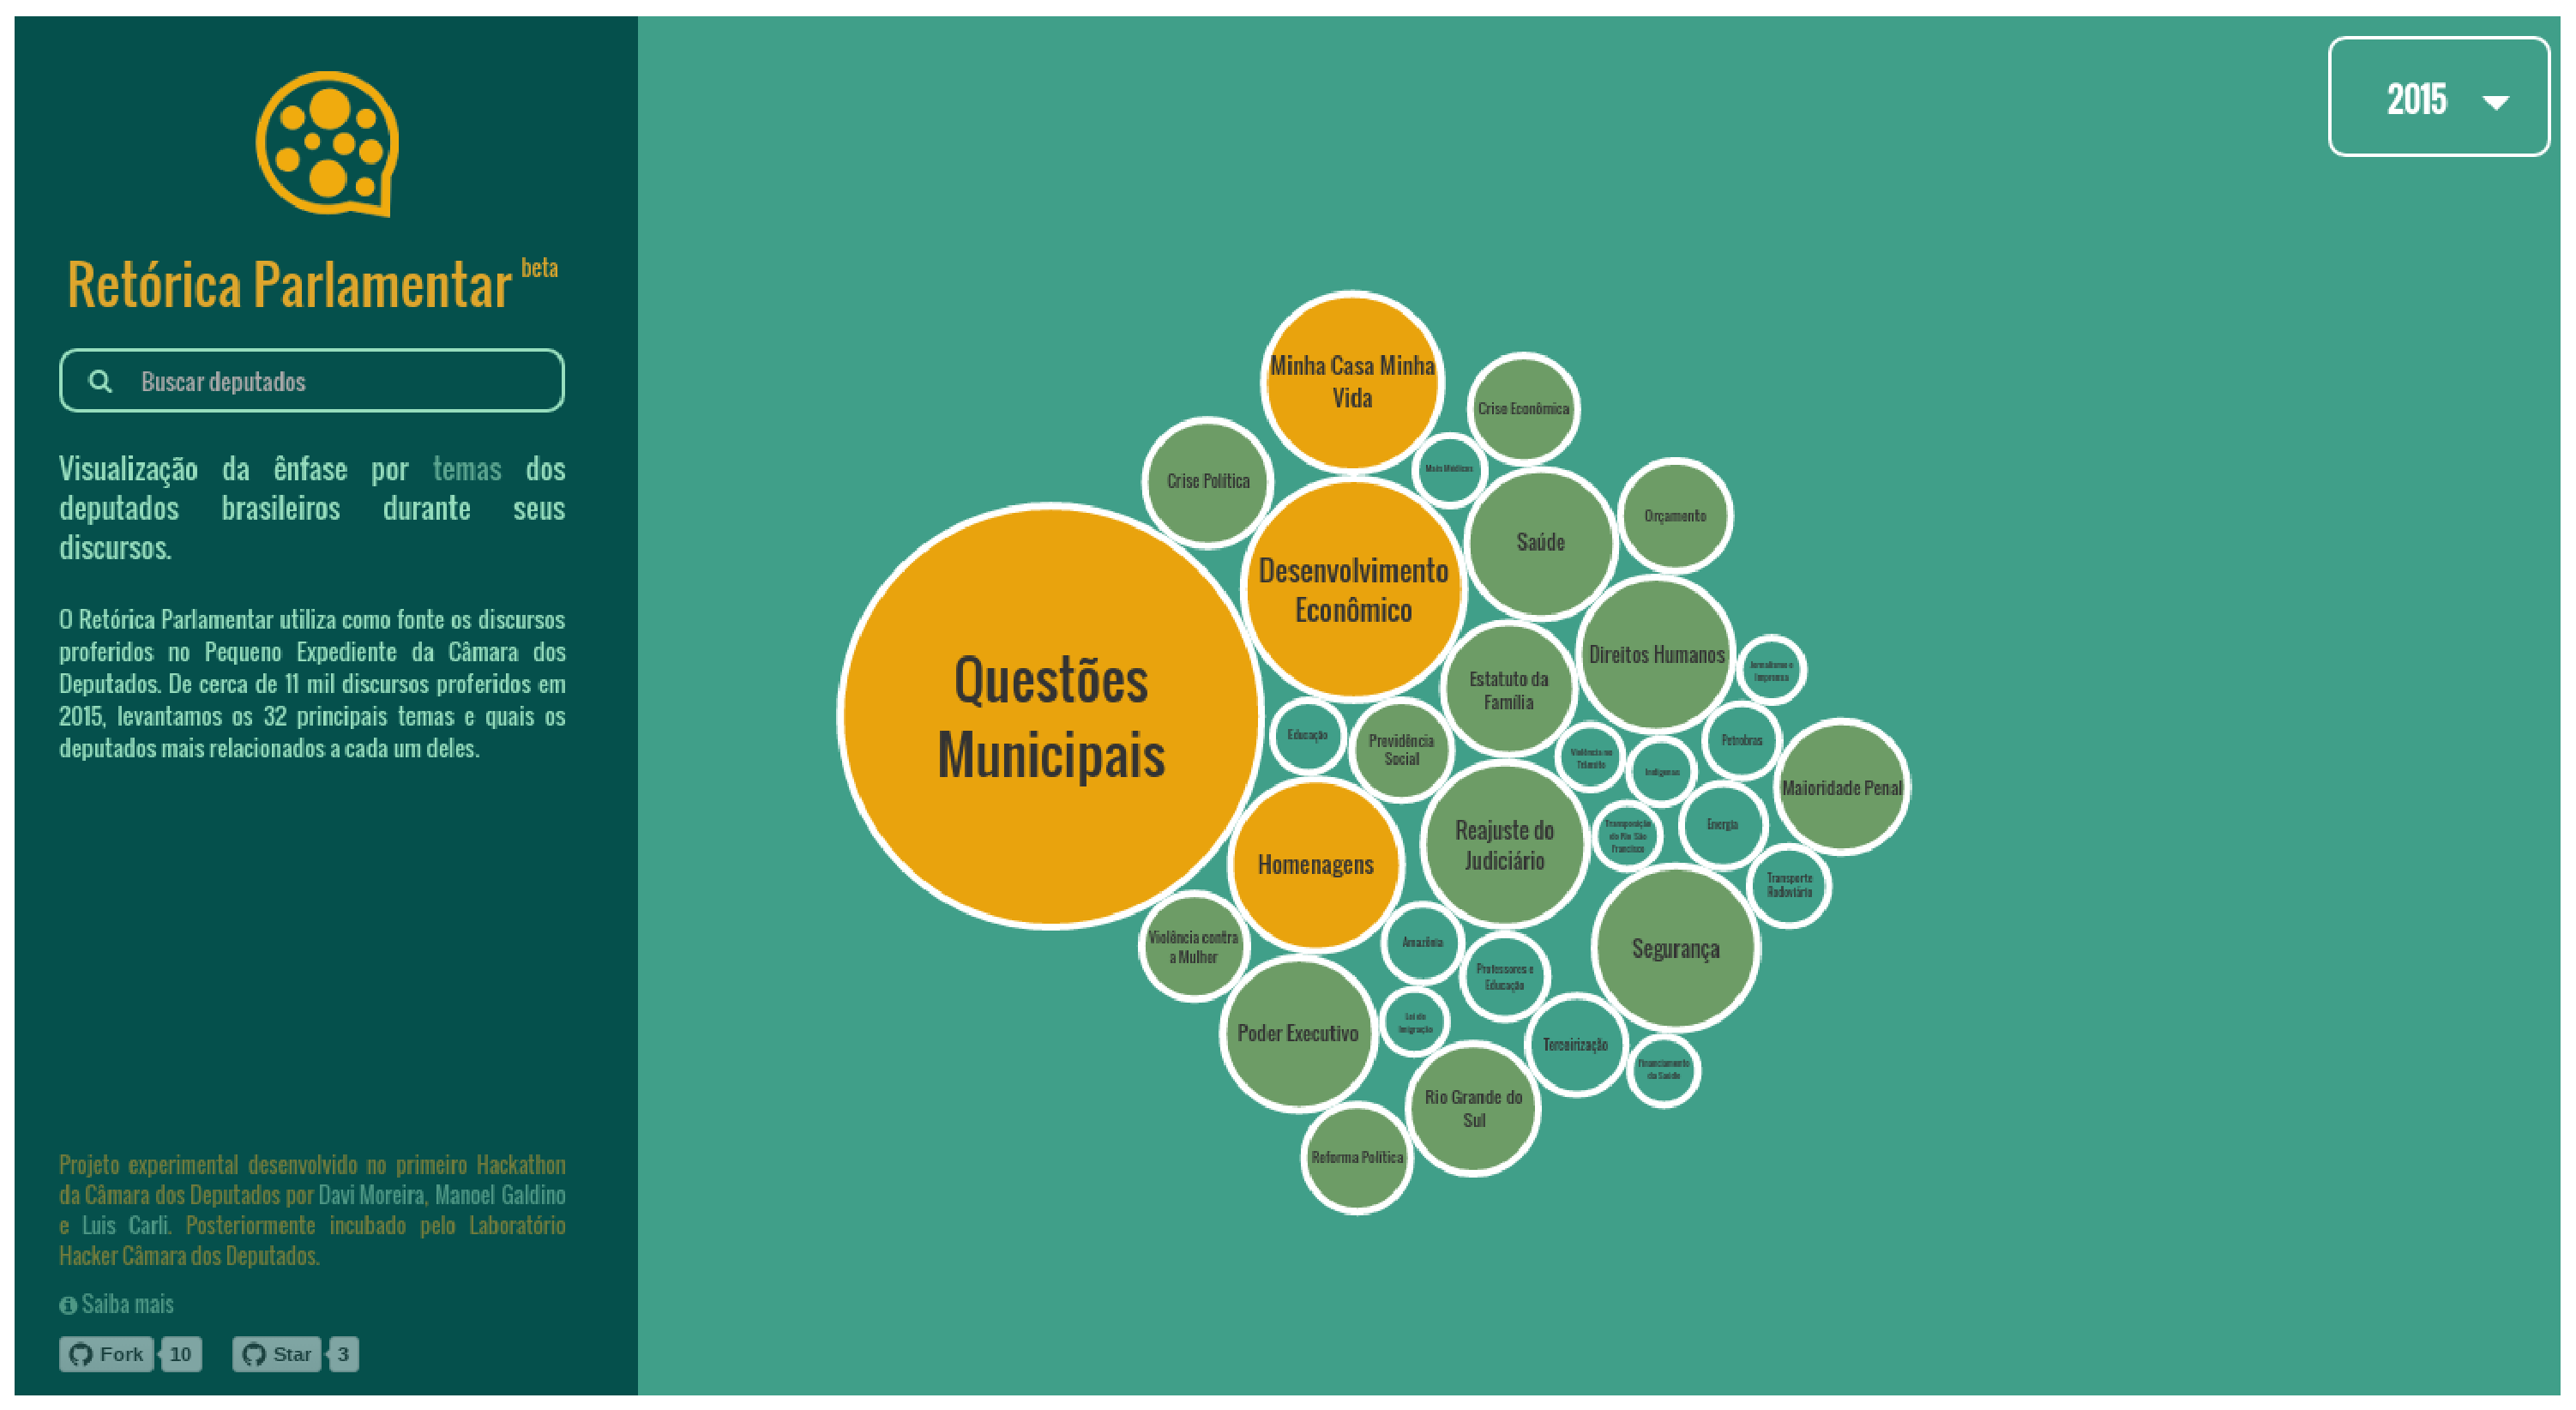
\includegraphics[scale=0.3]{figuras/retorica.eps}
    \caption{Retórica Parlamentar}
\end{figure}
